	\documentclass[12pt, a4paper]{report}
\usepackage{amsmath}
\usepackage{cclicenses}
\usepackage[hmargin=2.0cm, vmargin=1.5cm]{geometry}
\author {My\_WoRk\_\LaTeX\ \\ \\ HEMANT GORAKSH GHUGE \\\byncsa}
\title {LINUX}
\date {\today  \\first created on 8 June 2017 \\ last modified on 22 June 2017}
\pagestyle{headings}
\usepackage{hyperref}
\begin{document}
\maketitle
\pagenumbering{roman}
\setcounter{page}{2}
\tableofcontents
%
\chapter{Ubuntu-Desktop}
\pagenumbering{arabic}
\section{Learning Objectives}
\begin{enumerate}
\item ULD on gnome
\item Some applications in Ubuntu Desktop
\item Changing the theme of the Desktop
\end{enumerate}
\section{Terminal(command line)}
In fact, it is more powerful than the GUI\\
\\
\begin{tabular}{|lcr|}\hline
\$ ls && list \\ \hline
\end{tabular}
\section{Firefox Web Browser}
F6 - go to address bar\\
http://spoken-tutorial.org/
\section{Desktop}
$ctrl+windows+D$
\section{Summary}
\begin{enumerate}
\item Ubuntu Desktop
\item The launcher and some icon visible on it
\begin{enumerate}
\item Application
\item Calculator
\item Text Editor
\item Movie Player
\item LibreOffice Suite
\end{enumerate}
\end{enumerate}
%
\chapter{Desktop-Customization}
\section{Learning Objectives \& Summary}
\begin{enumerate}
\item about the launcher
\item remove and add application in the launcher
\item use multiple desktop
\item internet connectivity
\item sound settings
\item date \& time settings
\item switch to other user account
\end{enumerate}
%
\chapter{Synaptic-Package-Manager}
\begin{enumerate}
\item It is not a pre-installed application, has to be downloaded from Ubuntu Software Center.
\item Install, remove and upgrade software packages in user friendly way.
\item Synaptic is graphical package management tool based on GTK+ and APT.
\item Besides this basic function these features are provided:
\begin{enumerate}
\item Search and filter the list of available packages
\item Perform smart system upgrades
\item Fix broken package dependencies
\item Edit the list of used reposities(source.list)
\item Download the latest changelog of a package
\item Configure packages through the debconf system
\item Browse all available documentation relatedto a package(dwww is required)
\end{enumerate}
\end{enumerate}
%
\chapter{Ubuntu-Software-Center}
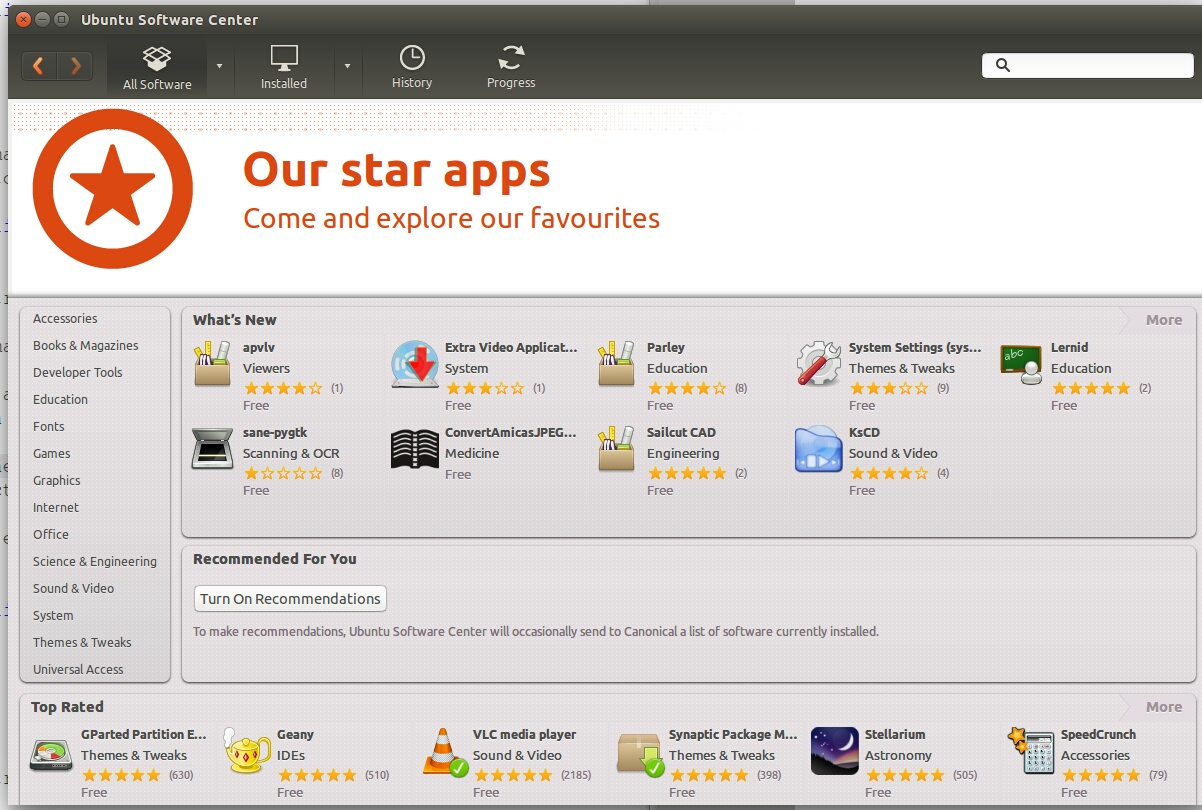
\includegraphics[width=\textwidth, angle=0]{04_usc.jpg}
\centerline{Figure 1: Ubuntu-Software-Center}
%
\chapter{Basic-Commands}
\section{What are Commands?}
\begin{enumerate}
\item words that when keyed in cause some action take p
\item Seldom more than four characters in length like ls, who, ps
\item Lower case
\item Case sensitive
\end{enumerate}
\begin{tabular}{|lcr|}\hline
\$ who && who is logged in \\ \hline
\end{tabular}
\section{Command Interpreter / Shell}
\begin{enumerate}
\item Program that act as the interface between us and the Linux system
\item Allow us to enter command for the operating system to execute
\item Multiple shell
\item Standard shell in Linux
\begin{enumerate}
\item Bash shell
\end{enumerate}
\item Other shells
\begin{enumerate}
\item Bourne shell (sh)
\item C shell (csh)
\item Korn shell (ksh)
\end{enumerate}
\end{enumerate}
\begin{tabular}{|lcl|}\hline
\$ echo \$SHELL && to see which shell is used\\
\$ type ps && this shows where ps command is stored\\
\$ echo \$PATH && \\ \hline
\end{tabular}
\section{Types of Commands}
\subsection{External Commands}
\begin{enumerate}
\item separate files/program
\item Eg : most commands like ls, ps etc
\end{enumerate}
\subsection{Internal Commands}
\begin{enumerate}
\item Implementation written within the shell
\item Do not exist as separate file
\item Eg : echo etc
\end{enumerate}
\begin{tabular}{|lcr|}\hline
\$ type echo && echo is shell builtin\\ \hline
\end{tabular}
\section{Structure of Commands}
\begin{enumerate}
\item One word or multiple words separated from white spaces
\item Multiple word case
\begin{enumerate}
\item First word - the actual name of the command
\item Other words - arguments
\end{enumerate}
\item Arguments - options or expression or filenames
\item A command can perform different task depending on the option specified
\item Short and long option
\end{enumerate}
\begin{tabular}{|l|}\hline
\$ ls\\
\$ ls -a\\
\$ ls -d\\
\$ ls --all
\\ \hline
\end{tabular}
\section{man Command}
\begin{enumerate}
\item System's Manual Pager
\item Argument - name of a program, utility or function.
\end{enumerate}
\begin{tabular}{|lcl|}\hline
\$ man man&&\\
\$ man -k directories && if confused which command to use\\
\$ apropos directories && copy above\\
\$ whatis ls&&\\
\$ ls --help&&\\ \hline
\end{tabular}
%
\chapter{General Purpose Utilities}
\begin{tabular}{|l|}\hline
\$ echo Hello World\\
\$ echo \$SHELL\\ \hline
\end{tabular}
\section{Common escape sequences with echo command}
\begin{enumerate}
\item We need to use the -e option of echo command for using escape sequences 
\begin{enumerate}
\item $\backslash$t for tab 
\item $\backslash$n for newline
\item $\backslash$c for displaying pr	ompt on the same line after message has been echoed
\end{enumerate}
\end{enumerate}
\begin{tabular}{|lcl|}\hline
\$ uname -r && what Kernel version you are using\\
\$ who am I && user name\\
\$ passwd && password change\\ \hline
\end{tabular}
\section{The Root User}
\begin{enumerate}
\item He is a special user with extra privileges
\item A root user is similar to a user in Windows with Administrator status\\
\\
\begin{tabular}{|l|}\hline
\$ date\\
\$ date +\%T \\
\$ date +\%h \\
\$ date +\%m \\
\$ date +\%y \\
\$ date +\%"\%h\%y" \\
\\
\$ cal\\
\$ cal 12 2017\\ \hline 
\end{tabular}
\item command 'pwd' \& 'echo \$HOME' are used for same thing i.e. present working directories\\
\end{enumerate}	
\begin{tabular}{|lcl|}\hline
\$ ls &&\\
\$ ls -all && all files including hidden\\
\$ ls -l && file permission, file owner name, last modification time, file size etc.\\
\$ ls -l $>$ fileinfo && redirects info into filename fileinfo\\ \hline
\end{tabular}\\
\\
\\
\begin{tabular}{|l|}\hline
\$ cat info\\
\\
\$ cat $>$ file\\
then write what you what to save\\
for save\&quit ctrl+d\\
for only quit ctrl+c\\
\\
\$ cat $>>$file \\ \hline
\end{tabular}
%
\chapter{File System}
\section{File}
\begin{enumerate}
\item In real life we know that a file is where we store our documents and papers.
\item Similarly in Linux a file is a container for storing information.
\end{enumerate}
\section{Directories}
\begin{enumerate}
\item A collection of files and other (sub)directories.
\item It gives:
\begin{enumerate}
\item Systematic storage of files.
\item Better protection and access control
\item Easier naming scheme for files
\end{enumerate}
\end{enumerate}
\section{File Inode}
\begin{enumerate}
\item Along with its contents, a file has a name and some properties, like:
\begin{enumerate}
\item The files creation/modificatio date, owner, size, its permissions where on the disk its stored
\end{enumerate}
\item The properties are stored in the files inode, a special block of data in the system.
\item A directory is a file that holds the inode nj=umbers and names of other files.
\end{enumerate}
\section{Types of Files}
\begin{enumerate}
\item In Linux ther are three kinds of files:
\begin{enumerate}
\item Regular Files or Ordinary files
\item Directories
\item Devices Files
\begin{enumerate}
\item helps to read from and write to devices in a way similar to that for ordinary files.
\end{enumerate}
\end{enumerate}
\end{enumerate}
\section{All files in Linux are related}
\begin{enumerate}
\item A directory containing files and subdirectories have a parent child relationship with each other.
\item Linux File System Tree
\item At the top is the root (denoted by frontslash /).
\item Easy navigation from one file or directory to other.
\end{enumerate}
\section{Home directory and Current directory}
\begin{enumerate}
\item When we login into the Linux system we are by default in a home directory.
\item The pwd command helps us to see the current directory.
\end{enumerate}
\begin{tabular}{|l|}\hline
\$ echo \$HOME \\
\$ pwd \\ \hline
\end{tabular}
\section{Change Directory(cd)}
\begin{enumerate}
\item We can move from one directory to other.The cd command is used for this.\\
\\
\begin{tabular}{|l|}\hline
\$ cd /usr\\
\$ pwd \\ \hline
\end{tabular}
\item Absolute Pathnames and Relative Pathnames
\item . represents current directory
\item .. represents the parent of the current directory\\
\\
\begin{tabular}{|l|}\hline
\$ cd\\
\$ cd Music\\
\$ pwd\\
\$ cd ..\\
\$ pwd\\
\$ cd ./Documents/\\
\$ pwd\\
\$ cd\\
\$ pwd\\ \hline
\end{tabular}
\item root\\
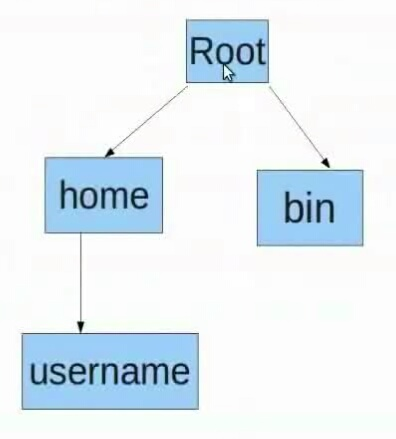
\includegraphics[width=0.25\textwidth]{07_fs.jpg}\\
Figure 2: root
\item How to change directory to bin?\\
\\
\begin{tabular}{|l|}\hline
\$ cd ../../bin\\
\$ pwd\\
\$ cd\\ \hline
\end{tabular}
\end{enumerate}
\section{The rmdir command}
Used to create a directory\\
\\
\begin{tabular}{|l|}\hline
\$ mkdir testdir \\
\$ mkdir test1 test2\\
\$ mkdir testtree testtree/test3\\ \hline
\end{tabular}
\section{The rmdir command}
\begin{enumerate}
\item Used to removing a directory or directories.
\item A directories can be removed by us only 
\begin{enumerate}
\item if we are its owner
\item our current directory is hierarchically above the directory to be removed
\item the directory is empty
\end{enumerate}
\end{enumerate}
\begin{tabular}{|l|}\hline
\$ rmdir test1\\
\$ cd testtree/test3\\
\$ rmdir testdir\\
\$ cd ..\\
\$ cd ..\\
\$ rmdir testdir\\
\$ rmdir testtree testtree/test3\\
\$ cd testtree\\
\$ ls\\ \hline
\end{tabular}
%
\chapter{Working with Regular Files}
\section{The cp command}
\begin{enumerate}
\item To copy a file from one place to another\\
\\
\begin{tabular}{|l|}\hline
\$ cp [OPTION]... SOURCE DEST\\
\$ cp [OPTION]... SOURCE(s)... DIRECTORY\\ \hline
\end{tabular}		
\item It copies SOURCE to DEST, or multiple SOURCE(s) to DIRECTORY
\end{enumerate}
\begin{tabular}{|l|}\hline
\$ cat test1\\
\$ cp test1 test2\\
\$ cat test2\\
\$ cp /home/anirban/arc/demo1 /home/anirban/arc/demo2\\
\$ ls /home/anirban\\
\$ cp /home/anirban/arc/demo1 /home/anirban/\\
\$ ls /home/anirban\\
\$ cp test1 test2 test3 /home/anirban/testdir\\
\$ ls /home/anirban/testdir\\ \hline
\end{tabular}
\section{The cp command option}
\begin{enumerate}
\item -R: For recursively copying directories\\
\\
\begin{tabular}{|l|} \hline
\$ cp testdir/ test\\
error\\
\$ cp -R testdir/ test\\
\$ ls\\
\$ clear\\
\$ ls test \\ \hline
\end{tabular}	
\item -b: For backup
\item -i: (interactive), warns us before overwriting any destination file
\end{enumerate}
\section{The mv command}
\begin{enumerate}
\item This is used for moving files.
\item It has two major uses.
\begin{enumerate}
\item Rename a file or directory
\item Moves a group of files to  different directory.
\end{enumerate}
\end{enumerate}
\begin{tabular}{|l|}\hline
\$ mv test1 test2\\
\$ mv -i anirban test2\\
\$ ls\\
\$ mv abc.txt pop.txt push.txt testdir\\
\$ ls testdir\\ \hline
\end{tabular}
\section{The mv command options}
\begin{enumerate}
\item -b: For backup, it will backup every file in the destionation before it is overwritten.
\item -i: (interactive), warns us before overwriting any destination file
\end{enumerate}
\section{The rm command}
\begin{enumerate}
\item This command is used for deleting files.
\item It can delete a single file as in\\
\\
\begin{tabular}{|l|}\hline
\$ rm testdir/faq.txt\\ \hline
\end{tabular}
\item or multiple files as in:\\
\\
\begin{tabular}{|l|}\hline
\$ rm testdir/abc1 testdir/abc2 \\ \hline
\end{tabular}	
\item Options
\begin{enumerate}
\item -r may be right protected
\item -f force delete\\
\\
\begin{tabular}{|l|}\hline
\$ rm testdir\\
error rm: cannot remove\\
\$ rm -rf testdir\\ \hline
\end{tabular}
\end{enumerate}
\end{enumerate}
\section{The cmp command}
\begin{enumerate}
\item Compares two files byte by byte.
\begin{enumerate}
\item Same content -$>$ no message
\item Different content -$>$ location of the first mismatch is printed\\
\\
\begin{tabular}{|l|}\hline
\$ cmp file1 file2\\
\$ cat sample1\\
\$ cat sample2\\
\$ cmp sample1 sample2\\
\$ clear\\ \hline
\end{tabular}
\end{enumerate}
\end{enumerate}
\section{The wc command}
\begin{tabular}{|lcr|} \hline
\$ cat sample3 && \\
\$ wc sample3 && lines, words, characters\\
6 67 385&&\\ \hline
\end{tabular}
%
\chapter{File Attributes}
\section{What is File Attribute?}
\begin{enumerate}
\item A file attribute is metadata that describes or is associated with computer file
\item File attribute is the characteristics that describe a file, such as owner, file type, access permissions, etc.
\end{enumerate}
\section{Changing Ownership}
\begin{enumerate}
\item chown command is used to change the ownership of the file or directory. Only administrator or root user can change the owner of a file or directory.
\item The syntax of chown command is\\ 
\\
\begin{tabular}{|l|}\hline
\$ chown [option] ownername filename/directoryname\\ \hline
\end{tabular}
\item -R : To change the permission on files that are in the subdirectories of the directory
\item -c : Change the permission for each file.
\item -f : Prevents chown from displaying error messages
\end{enumerate}
\begin{tabular}{|l|}\hline
\$ cd Desktop/file\_attr\\
\$ ls -l testchown\\
\$ sudo su chown -R anusha test\_chown\\
\$ ls -l\\ \hline
\end{tabular}
\section{chmod command}
\begin{enumerate}
\item chmod command is used to change the access mode (permissions) of one or more files.
\item syntax of the chmod command is \\
\\
\begin{tabular}{|l|}\hline
\$ chmod [options] mode filename \\ \hline
\end{tabular}
\item we may give the following options with chmod command.
\item-c, --changes : Print information about files that are changed.
\item -f, --silent, --quiet : Do not notify user of files that chmod cannot change.
\end{enumerate}
\section{File Permissions}
r : Read\\
w : Write\\
x : Execute\\
s : Set user (or group) ID\\\\
Alternatively, we may specify permissions by a three-digit octal number.\\
1st digit : owner permissions\\
2nd digit : group permissions\\
3rd digit : other permissions\\\\
4 : Read\\
2 : Write\\
1 : Execute\\
\\
\begin{tabular}{|l|}\hline
	\$ chmod u+x example1\\
	\$ ls -l example1\\
	\$ chmod 751 example1\\
	\$ ls -l example1\\
	\$ chmod =r example1\\
	\$ ls -l example1\\
	\$ chmod -R 755 directory1\\
	\$ ls -1\\
	\$ chmod u+x example2\\
	\$ ls -l example2\\
	\$ chmod g+w example3\\
	\$ ls -l example3\\
	\$ chmod a-w example3\\
	\$ ls -l example3\\ \hline
\end{tabular}
\section{Changing Group}
\begin{enumerate}
\item chgrp command is used to change the group of one or more files to new group.
\item The syntax for the chgrp command is \\
\\
\begin{tabular}{|l|}\hline
\$ chgrp [options] newgroup files\\ \hline
\end{tabular}
\end{enumerate}
\begin{tabular}{|l|}\hline
\$ ls -l example4\\
\$ sudo chgrp rohit example4\\
\$ ls -l example4\\ \hline
\end{tabular}
\section{Inode in Linux}
\begin{enumerate}
\item The inode number is a unique integer assigned to the device.
\item We can use ls -i command to see the inode number of a file.\\
\\
\begin{tabular}{|l|}\hline
\$ ls -i example5 \\ \hline
\end{tabular}
\end{enumerate}
\section{Hard Links}
\begin{enumerate}
\item Inodes are associated with precisely on directory entry at a time.
\item Hard links are to associate multiple directory entries with a single inode
\item ln is the command to make link
\item The syntax of ln command to create the hard link is\\
\\ 
\begin{tabular}{|l|}\hline
\$ ln source link\\ \hline
\end{tabular}
\item Where, source is an existing file and link is the file to create.
\end{enumerate}
\begin{tabular}{|l|}\hline
\$ clear\\
\$ ln example1 exampleln\\
\$ ls -i example1 exampleln\\ \hline
\end{tabular}
\section{Soft Links}
\begin{enumerate}
\item Soft link (symbolic link) is a special type of file that contains a reference to another file or directory in the form of an absolute or relative path.
\item The syntax of ln command to create the soft link is\\
\\ 
\begin{tabular}{|l|}\hline
\$ ln -s target-filename symbolic-filename\\ \hline
\end{tabular}
\end{enumerate}
\begin{tabular}{|l|}\hline
\$ ln -s example1 examplesoft\\
\$ ls -li example1 examplesoft\\ \hline
\end{tabular}
%
\chapter{Redirection \& Pipes}
\section{Stream :}
\begin{enumerate}
\item A Linux shell, such as Bash, receives input and output as sequences or streams of characters.
\item Accessed using file IO techniques.
\item Actual stream of characters may come from or go to a file
\end{enumerate}
\section{File Descriptor :}
\begin{enumerate}
\item Integer number
\item Associated with every open file of a process
\end{enumerate}
\section{The three standard streams}
\subsection{stdin}
\begin{enumerate}
\item It is the standard input stream
\item Provides input to commands
\item It has file descriptor 0
\end{enumerate}
\subsection{stdout}
\begin{enumerate}
\item It is the standard output stream
\item Provides output to commands
\item It has file descriptor 1
\end{enumerate}
\subsection{stderr}
\begin{enumerate}
\item It is the standard error stream
\item Provides error to commands
\item It has file descriptor 2
\end{enumerate}
\section{More about Streams}
\begin{enumerate}
\item Input streams provide input to programs
\item By default it takes from terminal keystrokes
	
\item Output streams print text characters
\item By default to the terminal -text window on a graphical desktop
	
\item we can change this default behaviour - Redirection
\end{enumerate}
\begin{tabular}{|lcl|}\hline
\$ wc && \\
\$ wc $<$ test1.txt && redirect stdin\\
\$ wc test1.txt && open the file \\ \hline
\end{tabular}
\section{Redirection- Two ways}
\subsection{n$>$}
\begin{enumerate}
\item Redirects output from file descriptor n to a file
\item Need write authority to the file
\item Destination file if does not exist - created
\item Destination file if existed - the existing contents are lost without any warning
\end{enumerate}
\subsection{n$>>$}
\begin{enumerate}
\item Redirects output from file descriptor n to a file
\item Need write authority to the file
\item Destination file if does not exist - created
\item Destination file if existed - the output is appended to the existing file
\end{enumerate}
IMP.
\begin{enumerate}
\item Redirects stdout $>$ or $>>$ (same as) 1$>$ or 1$>>$
\item Redirects stderr 2$>$ or 2$>>$
\end{enumerate}
\begin{tabular}{|l|}\hline
\# wc test1.txt $>$ wc\_results.txt\\
\# cat wc\_results.txt\\
\# wc test2.txt $>$ wc\_results.txt\\
\# cat wc\_results.txt\\
\\		
\# wc test1.txt $>>$ wc\_results.txt\\
\# cat wc\_results.txt\\
\\
\# wc aaa\\
\# wc aaa 2$>$ errorlog.txt\\
\# cat errorlog.txt\\
\\		
\# cat bbb 2$>$ errorlog.txt\\
\# cat errorlog.txt\\
\\		
\# wc aaa 2$>>$ errorlog.txt\\
\# cat errorlog.txt\\ \hline
\end{tabular}
\section{Pipes}
\begin{enumerate}
\item Manipulate and connect the different streams simultaneously.
\item Pipelining
\item Create chain of commands
\item Connects the output of one command to the input of the next command
\item It looks like\\
\\
\begin{tabular}{|l|}\hline
\# command1 $|$ command2 -option $|$ command3 -option1 -option2 $|$ command4\\ \hline
\end{tabular}
\end{enumerate}
\begin{tabular}{|l|}\hline\# ls -l\\
\# ls -l $>$ files.txt\\
\# wc -l files.txt\\
\# ls -l $|$ wc -l\\
\# cd /usr/bin\\
\# ls -l\\
\\
\# man ls\\ \hline
\end{tabular}
%
\chapter{Working with Linux Process}
\section{What is a process?}
\begin{enumerate}
\item	 Anything that is running in Linux is a process
\item Examples
\begin{enumerate}
\item Shell that is running and taking our commands
\item The commands that we type on terminal
\item Video in which you are seeing this tutorial
\item Browser in which you have opened the spoken-tutorial.org website
\item Shell scripts that are running
\end{enumerate}
\item A program which is being executed
\item Processes are much like us
\begin{enumerate}
\item They are born, they die
\item They have parent and children
\end{enumerate}
\end{enumerate}
\section{Shell process}
\begin{enumerate}
\item Shell is a process started by Linux Kernel as soon as we login to our system
\item The Linux Kernel is the core of the Linux operating system
\item Consists of the most essential component  that make Linux run
\item The shell creates or gives birth to all the other user command processes
\end{enumerate}
\begin{tabular}{|l|}\hline
\$ date \\ \hline
\end{tabular}
\section{Spawning}
\begin{enumerate}
\item A shell can also give birth to another shell process
\item Giving birth to a process or creating a process is also called spawning a process
\end{enumerate}
\begin{tabular}{|lcr|}\hline
\$ sh && given birth to new shell\\
\$ exit && \\ \hline
\end{tabular}
\section{Process attributes}
\begin{enumerate}
\item We are identified by attributes like our name, date of birth, etc
\item Similarly processes have attributes
\begin{enumerate}
\item PID: Process ID
\item PPID: Parent Process ID
\item Start time, etc
\end{enumerate}
\item PID: Each process is uniquely identified by an unique integer = PID
\item PPID: The PID of the parent of that process
\end{enumerate}
\begin{tabular}{|lcr|}\hline
\$ echo \$\$ && to check the PID of current shell\\ \hline
\end{tabular}
\section{ps command}
\begin{enumerate}
\item ps(process status) is a command which displays the processes running in the system
\item Let us see what happens if we run this command without any options
\end{enumerate}
\begin{tabular}{|lcr|}\hline
\$ ps&&\\
\$ sh&&\\
\$ ps&&\\
\$ ps -f && more attribute\\ \hline
\end{tabular}
\section{Process types}
\subsection{User processes}
\begin{enumerate}
\item Those processes that are started by the users
\item Eg: ps, most commands that we run on the terminal
\end{enumerate}
\subsection{System processes}
\begin{enumerate}
\item Those processes that are started
\begin{enumerate}
\item by the system often during system startup or
\item user login
\item Eg: bash
\end{enumerate}
\end{enumerate}
\section{All processes}
\begin{enumerate}
\item To see all the processes
\begin{enumerate}
\item System processes
\item User processes
\end{enumerate}
\item We use the -e or the -A option
\end{enumerate}
\begin{tabular}{|l|}\hline
\$ ps -e\\
\$ ps -e $|$ more\\ \hline
\end{tabular}
%
\chapter{The Linux Environment}
\section{Shell Variables}
\begin{enumerate}
\item Linux can be highly customized by changing the settings of the shell.
\item The behaviour of the shell is generally determined by the shell variables.
\end{enumerate}
\subsection{Environment Variables}
\begin{enumerate}
\item Available in user's total environment.
\item Also available in the sub-shells spawned by the shell (like the ones used for running shell scripts)
\end{enumerate}
\subsection{Local Variables}
\begin{enumerate}
\item Limited availability
\item Not available in the sub-shells spawned by the shell\\
\\
\begin{tabular}{|lcl|}\hline
\$ set $|$ more && Current Shell Variable \\
\$ env $|$ more  && Environment Variable\\ \hline
\end{tabular}
\end{enumerate}
\begin{tabular}{|lcl|}\hline
\$ echo \$SHELL&&\\
\$ echo \$HOME&&\\
\$ echo \$PATH&&\\
\$ PATH=\$PATH:/home/hemant/&&\\
\$ echo \$LOGNAME && stores user\_name of currently logged in user\\
\$ echo \$PS2 && it gives this'$>$' prompt changing '\$'\\
\$ PS1="@"&&\\
@&&\\
@ PS1="\$LOGNAME"&&\\
hemant&&\\
hemant&&\\
hemant PS1="\$"&&\\
\$&&\\
\$ && it is temporary\\
\$&&\\
\$ history&&\\
\$ history 10&&\\
\$ !593&&\\
\$ !! && last command\\
\$&&\\
\$ cd ~/testtree&&\\
\$ pwd&&\\
\$ cd -&&\\
\$ cd -&&\\
\$&&\\
\$&&\\
\$ alias cdMusic="cd /home/hemant/.../..."&&\\
\$ cdMusic&&\\
\$ pwd &&\\
/home/hemant/.../...&&\\
\$ cd -&&\\
\$ unalias cdMusic&&\\
\$ cdMusic && error\\
\$&&\\
\$ alias rm="rm -i"&&\\ \hline
\end{tabular}
%
\chapter{Basics of System Administration}
\section{Learning Objectives}
\begin{enumerate}
\item adduser
\item su
\item usermod
\item userdel
\item id
\item du
\item df
\end{enumerate}
\section{Prerequisite}
\begin{enumerate}
\item 06-General-Purpose-Utilities
\item One must have admin access in order to execute some admin command
\end{enumerate}
\section{adduser}
\begin{enumerate}
\item The 'adduser' command will create a new user login for us along with authentication.
\item We can add any user account with the help of 'sudo' command
\end{enumerate}
\section{sudo}
\begin{enumerate}
\item sudo command allows the administrative user to execute a command as a super user
\item The sudo command has many options\\
\\
\begin{tabular}{|l|}\hline
\$ sudo adduser\\
\$ sudo adduser duck\\
\$ ls /home\\ \hline
\end{tabular}
\end{enumerate}
\section{su}
\begin{enumerate}
\item su stands for 'Switch User'
\item This command is useful in switching from current user to another user\\
\\
\begin{tabular}{|l|}\hline
\$ su - duck\\
\$ logout\\ \hline
\end{tabular}
\end{enumerate}
\section{usermod}
\begin{enumerate}
\item Enables a super user or root user to modify the settings of other user accounts:
\begin{enumerate}
\item Change the password to no password or empty password.
\item Show the date on which the user account will be disabled.
\end{enumerate}
\begin{tabular}{|l|}\hline
\$ sudo usermod -e 2012-12-27 duck\\ \hline
\end{tabular}
\end{enumerate}
\section{id}
\begin{enumerate}
\item id command is used to check the identities of all the "users and groups" on the system.
\item To know about the identity of the user, we use id -u.
\item To know about the identity of the group users, it is id -g.\\
\\
\begin{tabular}{|lcr|}\hline
\$ id && \\
\$ id -u && user id\\
\$ id -n -u && name of user\\
\$ id -g && group id\\
\$ id -G && \\ \hline
\end{tabular}
\end{enumerate}
\section{userdel}
\begin{enumerate}
\item We can delete the user account permanently with the help of the userdel command\\
\\
\begin{tabular}{|lcr|}\hline
\$ sudo userdel -r duck && user along with home directory\\
\$ ls /home/&&\\ \hline
\end{tabular}
\end{enumerate}
\section{df and du}
\begin{enumerate}
\item The df command gives a report on the free space available on the disk.
\item The du command gives a report on how much space a file has occupied\\
\\
\begin{tabular}{|lcr|}\hline
\$ df &&\\
\$ df -h && human readable amount\\
&&\\
\$ cd /home/ &&\\
\$ du -s *.txt &&\\
\$ du -ch *.txt &&\\ \hline
\end{tabular}
\end{enumerate}
\section{Summary}
\begin{enumerate}
\item adduser command to create a new user account.
\item su command to switch from one user to another user.
\item usermod command for changing the user account settings.
\item userdel command to delete the user account.
\item id command to know the information about user ids and group ids.
\item df command to check the file system size and its availability.
\item du command to check the space occupied by a file.
\end{enumerate}
%
\chapter{Simple Filters}
\# sudo su or su root
\section{Prerequisite}
Ability to use the mouse, Keyboard, Maximize \& Minimize button on a window.
\section{head command}
\begin{enumerate}
\item head command followed by file name to display first 10 lines of a file by default.
\item Create a file \& type these numbers 1, 2, 22, 2, 4, 6, 7, 8, 99, 10, 11, 12
\item Save the file as number.txt\\
\\
\begin{tabular}{|l|}\hline
\$ cat number.txt\\
\$ head number.txt\\
\$ head -n5 number.txt\\ \hline
\end{tabular}
\end{enumerate}
\section{tail command}
\begin{enumerate}
\item Displays last 10 lines of file by default\\
\\
\begin{tabular}{|l|}\hline
\$ tail number.txt\\
\$ tail -n5 number.txt\\ \hline
\end{tabular}
\item A log file contains events which took place in a system.
\item auth.log file maintains log for who logged in \& who logged out.
\item Most useful Option -f\\
\\
\begin{tabular}{|l|}\hline
\$ tail -f /var/log/auth.log\\ \hline
\end{tabular}
\end{enumerate}
\section{Common Linux log files names \& Usage}
\begin{enumerate}
\item /var/log/auth.log: Authentication logs
\item /var/log/message: General \& system related stuff
\item /var/log/kern.log: Kernel logs
\item /var/log/cron.log: Crond logs (cron job)
\item /var/log/maillog: Mail server logs
\item /var/log/httpd/: Apache access \& error logs
\item /var/log/mysqld.log: MySQL DB server log file
\end{enumerate}
\section{sort command}
\begin{enumerate}
\item As the name suggest will sort a file in ascending, descending order\\
\\
\begin{tabular}{|l|}\hline
\$ sort number.txt\\
\$ sort -n number.txt\\
\$ sort -r number.txt\\
\$ sort -r -n number.txt\\ \hline
\end{tabular}
\item It can also pull out unique numbers\\
\\
\begin{tabular}{|l|}\hline
\$ sort -run number.txt\\ \hline
\end{tabular}
\item Create a file with the shown contents
\item Let us sort based on the second column\\
\\
\begin{tabular}{|l|}\hline
\$ sort marks.txt -t " " -k2\\
\$ cat marks.txt\\ \hline
\end{tabular}
\end{enumerate}
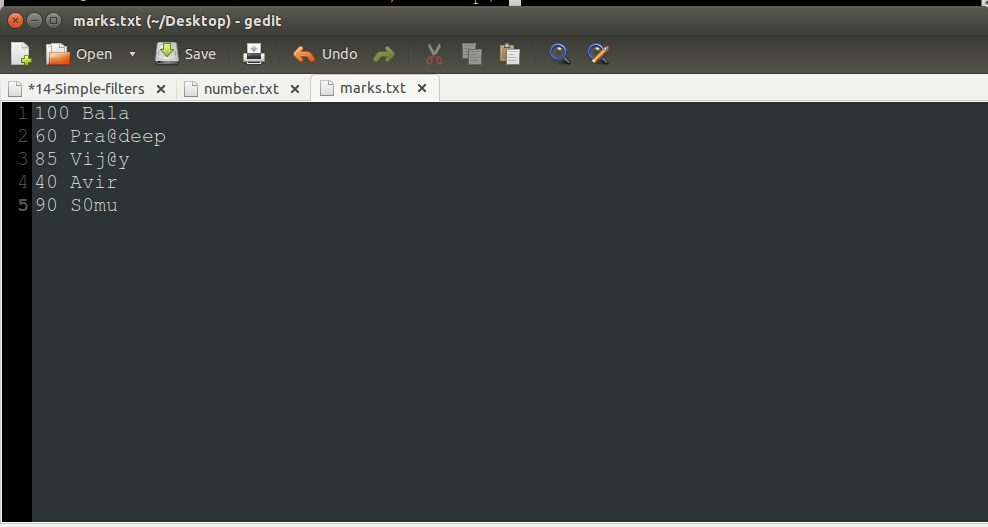
\includegraphics[width=\textwidth]{14_sf.jpg}\\
Figure 3: marks.txt
\section{cut command}
\begin{enumerate}
\item cut is used to cut certain information from a file
\item Let us pull out the names from marks.txt\\
\\
\begin{tabular}{|l|}\hline
\$ cut marks.txt -d " " -f2\\ \hline
\end{tabular}
\end{enumerate}
\section{paste command}
\begin{enumerate}
\item paste will merge lines of two or more files\\
\\
\begin{tabular}{|l|}\hline
\$ paste number.txt marks.txt\\ \hline
\end{tabular}
\item Redirects it to a new file\\
\\
\begin{tabular}{|l|}\hline
\$ paste number.txt marks.txt > concatfile.txt\\
\$ cat concatfile.txt\\ \hline
\end{tabular}
\item Print numbers serially\\
\\
\begin{tabular}{|l|}\hline
\$ paste -s number.txt\\ \hline
\end{tabular}
\end{enumerate}
\chapter{The grep command}
\$ bash -v
\section{Regular Expression}
\begin{enumerate}
\item Regular expressions are pattern matching techniques
\item To kind out whether a pattern exist in a line, paragraph or a file
\item For ex. If you want to search a phone number in the telephone directory\\ 
OR\\
To find a keyword in a paragraph or a line, we use grep command
\end{enumerate}
\section{Introduction to grep}
\begin{enumerate}
\item grep searches for one or more patterns in one or more line, paragraph or a file
\item If filename is not mentioned grep searches for the patterns in standard input
\item If filename is missing, grep searches for the patterns in the standard input
\end{enumerate}
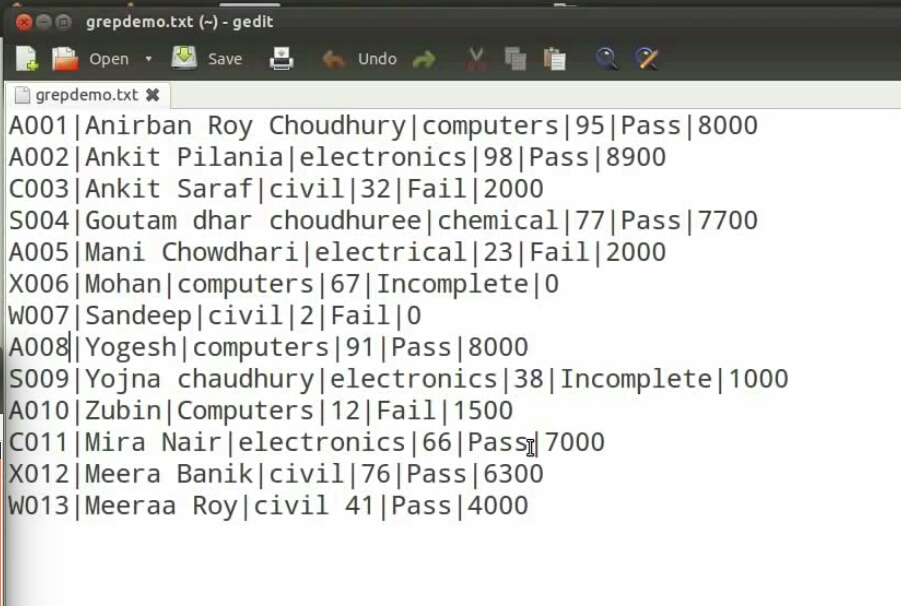
\includegraphics[width=0.8\textwidth]{15_grep.jpg}\\
Figure 4: grepdemo.txt\\
\begin{tabular}{|lcl|}\hline
\$ grep "computers" grepdemo.txt &&\\
\$ grep -i "computers" grepdemo.txt && includes C\\
\$ grep -iv "pass" grepdemo.txt $>$ notpass.txt && v is for not "   "\\
\$ cat notpass.txt &&\\
\$ grep -i "fail" grepdemo.txt &&\\
\$ grep -in "fail" grepdemo.txt && n number\\
\$ grep -i "ankit saraf" grepdemo.txt &&\\
\$ grep -i "fail" grepdemo.txt notpass.txt &&\\
\$ grep -c "Fail" grepdemo.txt && c count\\ \hline
\end{tabular}
\section{Summary}
\begin{enumerate}
\item To see the content of a file\\
\\
\begin{tabular}{|l|}\hline
\$ cat filename\\ \hline
\end{tabular}
\item To list the entries of a particular stream\\
\\
\begin{tabular}{|l|}\hline
\$ grep "computers" grepdemo.txt\\ \hline
\end{tabular}
\item To ignore cases\\
\\
\begin{tabular}{|l|}\hline
\$ grep -i "computers" grepdemo.txt\\ \hline
\end{tabular}
\item Lines that do not match the pattern\\
\\
\begin{tabular}{|l|}\hline
\$ grep -iv "pass" grepdemo.txt\\ \hline
\end{tabular}
\item To list the line numbers with the entries\\
\\
\begin{tabular}{|l|}\hline
\$ grep -in "fail" grepdemo.txt\\ \hline
\end{tabular}
\item To store the result in another file\\
\\
\begin{tabular}{|l|}\hline
\$ grep -iv "pass" grepdemo.txt $>$ notpass.txt\\ \hline
\end{tabular}
\item To know the count\\
\\
\begin{tabular}{|l|}\hline
\$ grep -c "Fail" grepdemo.txt\\ \hline
\end{tabular}
\end{enumerate}
\section{Assignment}
-E,+,?
\chapter{More on grep command}
\$ grep -e "electronics" -e "civil" grepdemo.txt\\
\$ grep -ie "chaudhury" -ie "chowdhari" grepdemo.txt
\section{Regular Expressions}
\begin{enumerate}
\item Provides a concise and flexible means for matching strings of text
\item Such as particular characters, words or patterns of characters	
\item There are a number of regular expression characters
\end{enumerate}
\section{The Character Class []}
\begin{enumerate}
\item Allows us to specify a group of characters within a pair of square brackets
\item Only one out of this group of characters is matched
\item Eg. [abc] would mean that this regular expression matches either a or b or c\\
\\
\begin{tabular}{|l|}\hline
\$ grep -i "ch[ao][uw]dh[ua]r[yi]" grepdemo.txt\\ \hline
\end{tabular}
\end{enumerate}
\section{Range}
\begin{enumerate}
\item If we want to specify a large range then write:
\item first letter dash last letter of the range
\item Suppose we like to match any digit we simply write [0-9]
\item One out of this group of characters is matched
\end{enumerate}
\section{The Asterisk}
\begin{enumerate}
\item The * refers to 0 or more occurrences of the immediately preceding character
\item For example ab* can match a, ab, abb, abbb etc.\\
\\
\begin{tabular}{|l|} \hline
\$ grep -i "m[ei]*raa*" grepdemo.txt\\
\$ grep "M... " grepdemo.txt\\
\$ grep "\^A" grepdemo.txt\\
\$ grep "[78]...\$" grepdemo.txt\\ \hline
\end{tabular}
\end{enumerate}
\section{Summary}
\begin{enumerate}
\item To match more than one pattern\\
\\
\begin{tabular}{|l|}\hline
\$ grep -e "electronics" -e "civil" grepdemo.txt\\ \hline
\end{tabular}
\item To check a word that has different spelling\\
\\
\begin{tabular}{|l|}\hline
\$ grep -ie "choudhury" -ie "chowdhari" grepdemo.txt\\ \hline
\end{tabular}
\item Character class\\
\\
\begin{tabular}{|l|}\hline
\$ grep -i "ch[ao][uw]dh[ua]r[yi]" grepdemo.txt\\ \hline
\end{tabular}
\item The use of Asterisk(*)\\
\\
\begin{tabular}{|l|}\hline
\$ grep -i "m[ei]*raa*" grepdemo.txt\\ \hline
\end{tabular}
\item To match any one character using dot\\
\\
\begin{tabular}{|l|}\hline
\$ grep "M... " grepdown.txt\\ \hline
\end{tabular}
\item To match a pattern at the beginning of the file\\
\\
\begin{tabular}{|l|}\hline
\$ grep "\^A" grepdemo.txt\\ \hline
\end{tabular}
\item To match a pattern at the end of the file\\
\\
\begin{tabular}{|l|}\hline
\$ grep "[78]...\$" grepdemo.txt\\ \hline
\end{tabular}
\end{enumerate}
\section{Assignment}
List those entries that are 5 letters long and starts with Y
%
\chapter{The sed command : The stream editor}
\section{Introduction to sed}
\begin{enumerate}
\item sed is a stream editor
\item sed finds some pattern of text in a particular location of a file
\item It performs some display or editing functions
\item Editing functions like:
\begin{enumerate}
\item Insertion
\item Substitution
\item Deletion of matched text
\end{enumerate}
\begin{tabular}{|l|}\hline
\$ cat seddemo.txt\\
OR\\
make a file seddemo.txt\\ \hline
\end{tabular}
\end{enumerate}
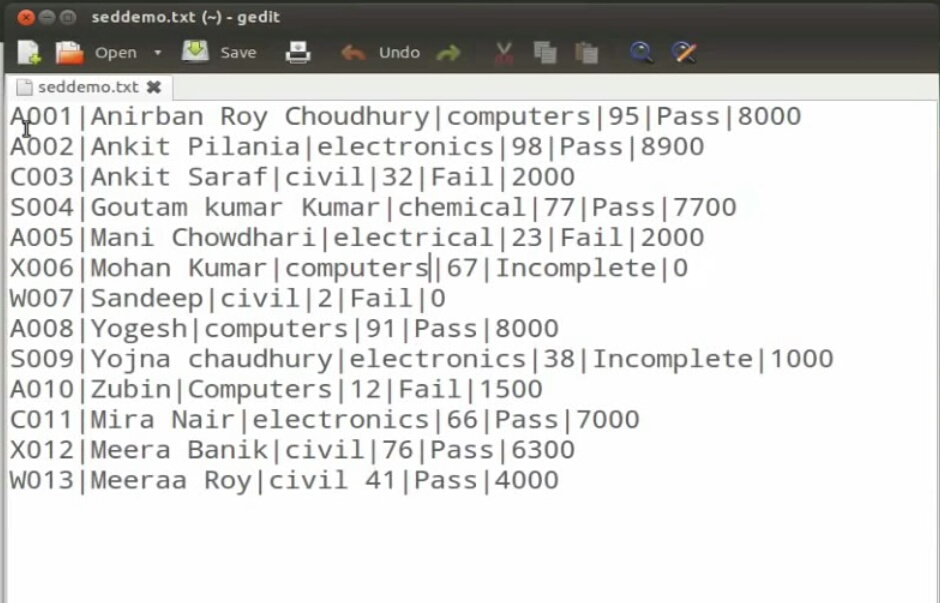
\includegraphics[width=0.8\textwidth]{17_sed.jpg}\\
Figure 5: seddemo.txt\\
\\
\begin{tabular}{|lcl|}\hline
\$ sed '2p' seddemo.txt && \\
\$ sed -n '2p' seddemo.txt	&& n silent mode, not print unnecessary output\\
\$ sed -n '\$p' seddemo.txt	&& \$ last line\\
\$ sed -n '3,6p' seddemo.txt && \\
\$ sed -n '3,6!p' seddemo.txt && ! except\\ \hline
\end{tabular}
\section{Line \& Context addressing}
\begin{description}
\item[Line Addressing]Address specified by the line number
\item[Context Addressing]Lines that contain particular context say a particular word.
\end{description}
\begin{tabular}{|lcr|}\hline
\$ sed -n '/[cC]omputers/p' seddemo.txt && \\
\$ sed -n '/[cC]omputers/w computer\_student.txt' seddemo.txt	&& w save file in filename.txt \\
\$ cat computer\_student.txt && \\
\$ sed -n -e 'electronic/w electro.txt' -e '/civil/w civil.txt' seddemo.txt && \\
\$ cat electro.txt && \\
\$ cat civil.txt && \\ \hline
\end{tabular}
\section{Summary}
\begin{enumerate}
\item sed
\item To print using sed
\item Line Addressing
\item Context Addressing
\end{enumerate}
\section{Assignment}
\begin{enumerate}
\item Use the same text file seddemo.txt
\item Try to print records from 6th to 12th line
\end{enumerate}
\chapter{More on sed command}
The major use of sed is substitution\\
Replacing some pattern in the input with something else
\section{Substitution \& Replacement}
\begin{tabular}{|lcr|}\hline
\$ sed 's/[kK]umar/Roy/' seddemo.txt && \\
\$ sed 's/[kK]umar/Roy/g' seddemo.txt	 &&  g everywhere\\
\$ sed -e 's/electronics/electrical/g' -e 's/civil/metallurgy/g' seddemo.txt && \\
\$ sed '/Anirban/s/computers/mathematics/g' seddemo.txt && \\
\$ sed '/electronics/d' seddemo.txt $>$ nonelectronics.txt && \\
\$ cat nonelectronics.txt && \\ \hline
\end{tabular}
\section{Insertion}
\begin{tabular}{|l|}\hline
\$ sed '1i Student Information' seddemo.txt\\
\$ sed '1i Student Information$\backslash$n2013' seddemo.txt\\ \hline
\end{tabular}
\section{Summary}
\begin{enumerate}
\item Substitution
\item Replacement
\item Insertion
\end{enumerate}
\section{Assignment}
\begin{enumerate}
\item Use the same text file seddemo.txt
\item Try to replace or substitute name Ankit with Ashish
\end{enumerate}
\chapter{Basics of awk}
\section{Introduction}
\begin{enumerate}
\item awk is a very powerful text manipulation tool
\item It is named after its authors Aho, Weinberger and Kernighan
\item It can perform several functions
\item It operates at the field level of a record
\item So, it can easily access and edit the individual fields of the record
\end{enumerate}
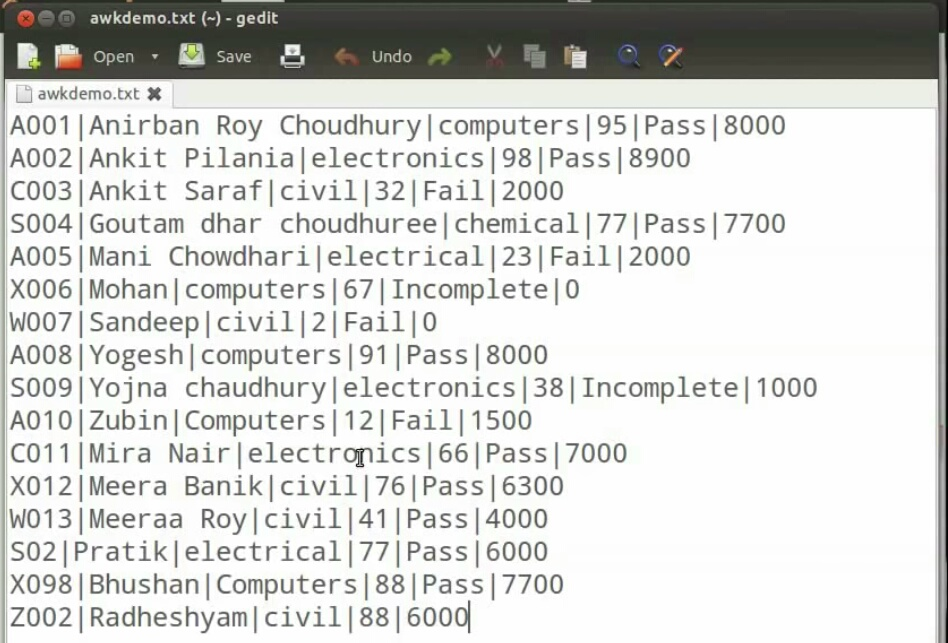
\includegraphics[width=0.8\textwidth]{19_awk.jpg}\\
Figure 6: awkdemo.txt\\
\\ \\
\begin{tabular}{|l|}\hline
\$ awk '/Pass/{print}' awkdemo.txt\\
\$ awk '/M[ei]*ra*/{print}' awkdemo.txt\\
\$ awk '/civil$|$electrical/ {print}' awkdemo.txt\\ \hline
\end{tabular}
\\ \\ 
\section{Parameters}
\begin{enumerate}
\item awk has some special parameters to identify individual fields of a line
\item \$1(Dollar 1) would indicate the first field
\item Similarly we can have $2, $3 and so on, for respective fields
\item \$0 represents the entire line
\item $|$   delimeter
\end{enumerate}
\begin{tabular}{|l|} \hline
\$ awk -F "$|$" '/civil$|$electrical/{print \$0}' awkdemo.txt\\
\$ awk -F "$|$" '/civil$|$electrical/{print \$2,\$3}' awkdemo.txt\\
\$ awk -F "$|$" '/Pass/{printf"\%4d \%-25s \%-15s $\backslash$n",NR,\$2,\$3}' awkdemo.txt\\ \hline
\end{tabular}
\section{Summary}
\begin{enumerate}
\item To print using awk
\item Regular expression in awk
\item To list the entries for a particular stream
\item To list only the second and the third fields
\item To display a formatted output
\end{enumerate}
\section{Assignment}
Display roll no., stream and marks of Ankit Saraf
\end{document}\grid
